\section{Theorie}

    Im Folgenden werden die theoretischen Grundlagen des Franck-Hertz-Versuches vorgestellt.\\
    \\
    Der Franck-Hertz-Versuch gehört zu den Elektronenstoßexperimenten,
    bei denen beschleunigte Elektronen auf Atome geschossen werden. %??
    Aus der Energiedifferenz der Elektronen können Informationen über die angeregten Zustände des Atoms gewonnen werden.


\subsection{Das Franck-Hertz-Experiment}
\label{sec:grundprinzip}

    % Für den Franck-Hertz-Versuch ist der folgende \hyperref[fig:aufbau]{Aufbau} gegeben.
    Für den Franck-Hertz-Versuch ist der in \autoref{fig:aufbau} schematisch dargestellte Aufbau gegeben.
    \begin{figure}[H]
        \centering
        \includegraphics[width=0.6\textwidth]{content/img/Abb_1.pdf}
        \caption{Aufbau des Franck-Hertz-Versuches. \cite{versuchsanleitung}}
        \label{fig:aufbau}
    \end{figure}
    Die Apparatur besteht aus einer evakuierten Röhre,
    in der sich ein Quecksilber-Tropfen befindet,
    der spontan verdampft, %TODO spontan!?
    sodass sich ein Gleichgewichtsdruck $p_\text{Sät}$ einstellt.
    Die Dampfdichte hängt ausschließlich von der Umgebungstemperatur $T$ ab
    und kann so kontrolliert werden.\\
    In der Röhre befindet sich außerdem eine negativ geladener Glühdraht,
    aus welchem durch den glühelektrischen Effekt Elektronen austreten.
    Er ist zusätzlich mit einem Material beschichtet,
    welches eine besonders geringe Austrittsarbeit besitzt,
    sodass möglichst viele freie Elektronen erzeugt werden können.
    % Somit sollten aus der Glühkathode auch deutlich mehr Elektronen ausgelöst werden als aus der →Auffängerelektrode?←
    Die Elektronen werden zu einer positiv geladenen Gitterelektrode hin beschleunigt,
    wobei zwischen Draht und Gitterelektrode die Beschleunigungsspannung $U_\text{B}$ anliegt.
    Wenn die Elektronen zu Beginn eine Geschwindigkeit von Null besitzen,
    gilt wegen der Energieerhaltung nach Durchlaufen des Feldes
    \begin{equation*}
        \frac{m_0}{2}v^2_\text{vor} = e_0 U_\text{B} \ .
    \end{equation*}
    \\
    Hinter der Gitterelektrode befindet sich eine Auffängerelektrode,
    welche negativ geladen ist.
    Zwischen Gitter- und Auffängerelektrode liegt eine Bremsspannung $U_\text{A}$ an.
    Es entsteht ein Gegenfeld,
    das die Elektronen überwinden müssen,
    um auf die Auffängerelektrode zu treffen,
    an der dann ein Auffängerstrom $I_\text{A}$ gemessen wird.
    Es kommen nur diejenigen Elektronen an der Auffängerelektrode an,
    deren Energie groß genug ist,
    um das Gegenfeld zu passieren.
    Es gilt
    \begin{equation}
        \frac{m_0}{2}v^2_\text{z} \geq e_0 U_\text{B} \ .
        \label{eqn:energie_gegenfeld}
    \end{equation}
    \\
    Im Bereich zwischen Glühdraht und Gitterelektrode kann es zu Stößen zwischen Elektronen und Quecksilber-,
    kurz $\ce{Hg}$-Atomen,
    kommen.
    Abhängig von der Beschleunigungsspannung $U_\text{B}$ wird zwischen zwei Möglichkeiten unterschieden.\\
    % → 1. (!?)
    \indent
    Zum einen ist Energie der Elektronen gerade bei niedriger Beschleunigungsspannung noch nicht groß genug,
    um die $\ce{Hg}$-Atome anzuregen,
    sodass es nur zu elastischen Stößen kommt,
    bei denen die Elektronen nicht viel Energie abgeben,
    aber ihre Richtung ändern können,
    aufgrund des Massenverhältnisses $\sfrac{m_0}{M}$ zwischen Elektronen und $\ce{Hg}$-Atomen von $\sfrac{1}{1836\cdot201}$.
    Die übertragene Energie beim elastischen Stoß beträgt
    \begin{equation*}
        \symup{\Delta}E = \frac{4 m_0 M}{(m_0 + M)^2} E \approx \num{1.1e-5} E
    \end{equation*}
    mit der Elektronenmasse $m_0$ und der $\ce{Hg}$-Atommasse $M$.\\
    % → 2. (!?)
    \indent
    Bei der zweiten Möglichkeit ist die Energie der Elektronen durch eine größere Beschleunigungsspannung groß genug,
    dass sie die $\ce{Hg}$-Atome anregen können.
    Dabei überträgt das Elektron den Energiebetrag $E_1 -E_0$ zwischen dem Grundzustand und dem ersten angeregten Zustand des $\ce{Hg}$-Atoms auf ein Elektron in einer inneren Hülle des Atoms.
    Das Elektron behält eine Restenergie von $E - (E_1 - E_0)$ zurück.
    Nach einer Relaxationszeit von etwa $\SI{e-8}{\second}$ kehrt das $\ce{Hg}$-Atom in den Grundzustand zurück und ein Photon mit der durch den Übergang freigewordenen Energie
    \begin{equation*}
        E_\text{Photon} = h \nu = E_1 - E_0
    \end{equation*}
    wird emittiert.\\
    Aus der Geschwindigkeitsänderung des Elektrons durch die Energieabgabe kann die Energiedifferenz zur Anregung bestimmt werden.
    Es gilt
    \begin{equation*}
        \frac{m_0 v^2_\text{vor}}{2} - \frac{m_0 v^2_\text{nach}}{2} = E_1 - E_0 \ .
    \end{equation*}
    \\
    Immer,
    wenn die Energie des Elektrons größer oder gleich der Anregungsenergie ist,
    hat es nach dem inelastischen Stoß nicht mehr genug Restenergie,
    um das Gegenfeld zwischen Gitter- und Auffängerelektrode zu überwinden,
    wodurch der Auffängerstrom sinkt.
    Dies ist in Abhängigkeit der Beschleunigungsspannung in \autoref{fig:idealer_verlauf} dargestellt,
    wobei dies nur den Verlauf unter idealen Bedingungen beschreibt.
    \begin{figure}[H]
        \centering
        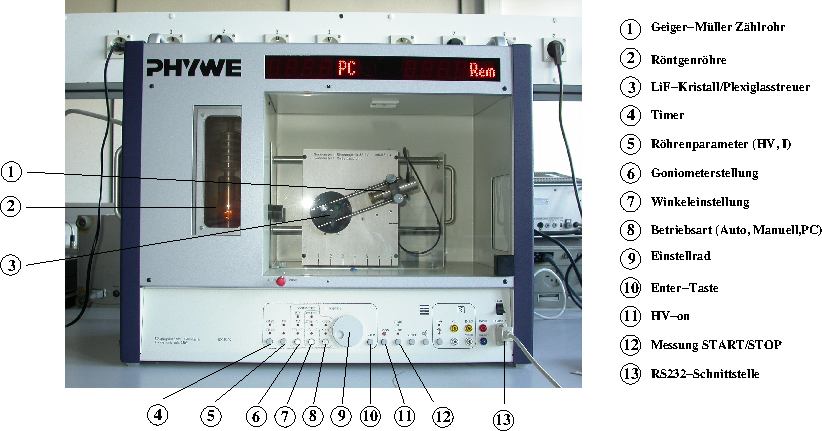
\includegraphics[width=0.5\textwidth]{content/img/Abb_2.pdf}
        \caption{Idealer Verlauf des Auffängerstroms in Abhängigkeit der Beschleunigungsspannung. \cite{versuchsanleitung}}
        \label{fig:idealer_verlauf}
    \end{figure}
    Zu Beginn ist die Beschleunigungsspannung noch gering,
    sodass keine Elektronen das Gegenfeld überwinden können.
    Der Auffängerstrom ist also gleich Null.
    Bei steigender Beschleunigungsspannung haben mehr Elektronen
    die zum Erreichen der Auffängerelektrode notwendige Energie,
    sodass der Strom $I_\text{A}$ ab dem Punkt steigt,
    bei dem $U_\text{B} > U_\text{A}$ gilt.
    Der Strom nimmt mit steigender Beschleunigungsspannung bis zu dem Punkt zu,
    an dem diese einen Wert von $U_1$ errreicht hat und die Elektronen die Energie $E_1-E_0$ besitzen.
    Nun werden die $\ce{Hg}$-Atome angeregt und der Auffängerstrom sinkt stark ab,
    wie oben gezeigt.
    Wenn die Beschleunigungsspannung nun weiter steigt,
    haben die Elektronen schneller die zum Anregen $\ce{Hg}$-Atome nötige Energie
    und die (im gegebenen Versuchsaufbau nicht sichtbare) Leuchtschicht wandert in Richtung des Glühdrahts.
    Zudem haben auch mehr Elektronen genug Energie,
    um das Gegenfeld zu überwinden,
    sodass auch die Peaks in der Stromstärke zunehmend intensiver werden.\\
    Dieser Vorgang setzt sich periodisch fort.
    Der Spannungsabstand $U_1$ entspricht der Anregungsenergie des $\ce{Hg}$-Atoms
    \begin{equation*}
      % TODO: Einheiten-Check?
        U_1 = \frac{1}{e_0} (E_1 - E_0)
    \end{equation*}
    mit der Elektronenladung $e_0$.


\subsection{Einflüsse auf den Verlauf der Franck-Hertz-Kurve}
\label{sec:einflüsse}

    Der in \autoref{fig:idealer_verlauf} dargestellte idealisierte Verlauf der Franck-Hertz-Kurve
    kann nicht realisiert werden,
    da verschiedene Nebeneffekte zu berücksichtigen sind,
    die den Verlauf beeinflussen.


\subsubsection{Das Kontaktpotential}
\label{sec:einflüsse:kontaktpotential}

    Ein Nebeneffekt kommt dadurch zustande,
    dass sich das Potential des Glühdrahtes von dem der Gitterelektrode unterscheidet.
    Bei gleichem Potential träten bei steigender Temperatur auch aus der Gitterelektrode Elektronen aus,
    welche die Messung verfälschen würden.
    % NOTE: Sicher in diese Richtung? Nicht von Auffängerelektrode zu Gitterelektrode (negativ → positiv)? Oder beides?
    % → Katharina sagt, das stimmt so. ¯\_(ツ)_/¯
    Deshalb wird der Glühdraht so beschichtet,
    dass er eine geringere Austrittsarbeit als die Gitterelektrode aufweist.\\
    Die Potentialverhältnisse sind in \autoref{fig:potentialverhältnisse} dargestellt.
    \begin{figure}[H]
        \centering
        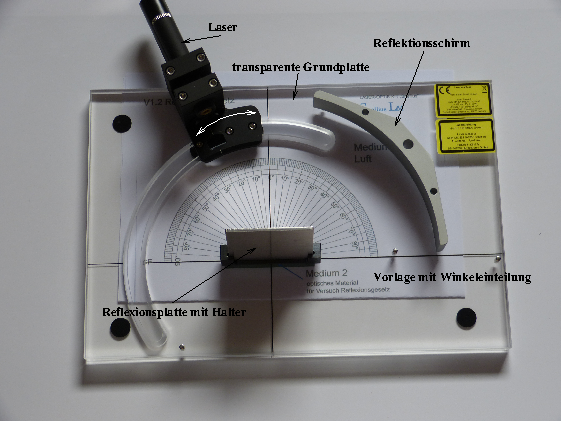
\includegraphics[width=0.9\textwidth]{content/img/Abb_3.pdf}
        \caption{Das Verhältnis zwischen dem Potential des Glühdrahtes und der Gitterelektrode. \cite{versuchsanleitung}}
        \label{fig:potentialverhältnisse}
    \end{figure}
    Die Größen $\Phi_\text{G}$ und $\Phi_\text{B}$ stellen die Austrittsarbeiten des Drahtes und der Gitterelektrode dar.\\
    Aus dem Potentialverhältnis ergibt sich ein Kontaktpotential
    \begin{equation*}
        % K = \frac{1}{e_0} (\Phi_\text{B} - \Phi_\text{G}) \ ,
        K = \frac{\Phi_\text{B}}{e_0} - \frac{\Phi_\text{G}}{e_0} \ ,
    \end{equation*}
    welches eine Verschiebung der Franck-Hertz-Kurve nach der Gleichung
    \begin{equation}
        U_\text{B,eff} = U_\text{B} - K
        \label{eqn:kontaktpotential_verschiebung}
    \end{equation}
    bewirkt.


\subsubsection{Die Energieverteilung der Elektronen}
\label{sec:einflüsse:energieverteilung}

    Ein weiterer Nebeneffekt entsteht durch die Fermi-Dirac-Verteilung der Elektronen im Glühdraht,
    welche aussagt,
    dass sich die Elektronen schon vor dem Herauslösen auf verschiedenen Energieniveaus befinden,
    sodass sie unterschiedliche Anfangsgeschwindigkeiten haben,
    wenn sie aus dem Draht gelöst werden,
    und somit nach der Beschleunigung ein kontinuierliches Energiespektrum besitzen.\\
    Es kann also kein einheitlicher Abstand $U_1$ zwischen den Strommaxima erreicht werden,
    da die Elektronen unterschiedlich stark beschleunigt werden,
    um bei inelastischen Stößen die $\ce{Hg}$-Atome anzuregen.
    Aus diesem Grund wird auch der Auffängerstrom nicht mehr ganz auf Null abfallen,
    sondern immer nur einen Minimalwert erreichen.\\
    \\
    Zudem ist die Richtungsänderung der Elektronen bei elastischen Stößen im Bereich zwischen der Gitterelektrode und der Auffängerelektrode relevant,
    da bei diesen Stößen die z-Richtung der Elektronen verändert wird,
    % Ungleichung \ref{eqn:energie_gegenfeld}
    woraus nach \hyperref[eqn:energie_gegenfeld]{Ungleichung \getrefnumber{eqn:energie_gegenfeld}} folgt,
    dass sie die Auffängerelektrode nicht mehr erreichen können.


\subsubsection{Der Dampfdruck}
\label{sec:einflüsse:dampfdruck}

    Ein weiterer Einfluss auf den Verlauf der Kurve ist durch den Dampfdruck $p_\text{Sät}$ gegeben,
    da der Franck-Hertz-Effekt nur messbar ist,
    wenn es zu genügend inelastischen Stößen zwischen Elektronen und $\ce{Hg}$-Atomen kommt.
    Dies ist gegeben,
    wenn die mittlere Weglänge $\bar{w}$ klein gegenüber dem Abstand $a$ zwischen Glühdraht und Gitterelektrode ist.\\
    Da der Dampfdruck ausschließlich von der Temperatur $T$ abhängig ist,
    können so die Temperaturen bestimmt werden,
    bei denen der Franck-Hertz-Effekt auftritt.\\
    Diese Abhängigkeit ist in \autoref{fig:dampfdruckkurve} gezeigt.
    \begin{figure}[H]
        \centering
        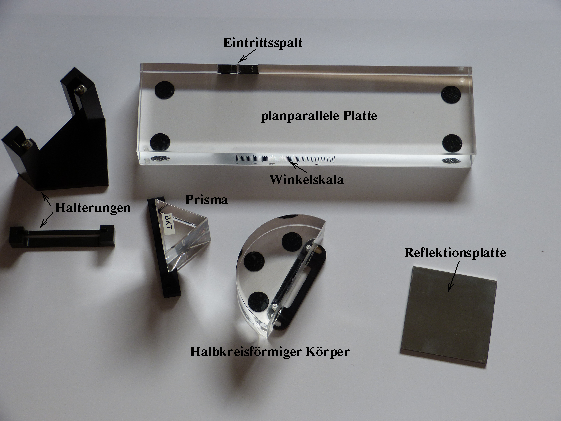
\includegraphics[width=0.35\textwidth]{content/img/Abb_4.pdf}
        \caption{Abhängigkeit des Dampfdrucks von $\ce{Hg}$ von der Temperatur. \cite{versuchsanleitung}}
        \label{fig:dampfdruckkurve}
    \end{figure}
